\let\negmedspace\undefined
\let\negthickspace\undefined
\documentclass[journal]{IEEEtran}
\usepackage[a5paper, margin=10mm, onecolumn]{geometry}
%\usepackage{lmodern} % Ensure lmodern is loaded for pdflatex
\usepackage{tfrupee} % Include tfrupee package

\setlength{\headheight}{1cm} % Set the height of the header box
\setlength{\headsep}{0mm}     % Set the distance between the header box and the top of the text

\usepackage{gvv-book}
\usepackage{gvv}
\usepackage{cite}
\usepackage{amsmath,amssymb,amsfonts,amsthm}
\usepackage{algorithmic}
\usepackage{graphicx}
\usepackage{textcomp}
\usepackage{xcolor}
\usepackage{txfonts}
\usepackage{listings}
\usepackage{enumitem}
\usepackage{mathtools}
\usepackage{gensymb}
\usepackage{comment}
\usepackage[breaklinks=true]{hyperref}
\usepackage{tkz-euclide} 
\usepackage{listings}
% \usepackage{gvv}        
\def\inputGnumericTable{}                                 
\usepackage[latin1]{inputenc}                                
\usepackage{color}                                            
\usepackage{array}                                            
\usepackage{longtable}                                       
\usepackage{calc}                                             
\usepackage{multirow}                                         
\usepackage{hhline}                                           
\usepackage{ifthen}                                           
\usepackage{lscape}

\begin{document}

\title{1.9.7}
\author{EE25BTECH11018 - Darisy Sreetej}
\maketitle

\textbf{Question:}\\
Find the distance of the point \brak{-6,8} from the origin.

\textbf{Solution:}\\
Let the given point be
\begin{align*}
    \vec{P} = \myvec{-6 \\ 8}
\end{align*}
The distance of the point from the origin is the length of its position vector $\vec{P}$. The formula is given as 
\begin{align}
\norm{\vec{P}} = \sqrt{\vec{P}^\top \vec{P}} \label{eq:1}
\end{align}

\begin{align*}
    \vec{P}^\top = \myvec{-6 & 8}
\end{align*}

From (1), we have
\begin{align}
    \vec{P}^\top \vec{P} &= \myvec{-6 & 8} \myvec{-6 \\ 8} \\
    &= \brak{-6}\brak{-6} + \brak{8}\brak{8} \\
    &= 36 + 64 \\
    &= 100
\end{align}

\begin{align*}
    \text{Distance} = \norm{\vec{P}} = \sqrt{\vec{P}^\top \vec{P}} = \sqrt{100} = 10
\end{align*}

$\therefore$ The distance of the point \brak{-6, 8} from the origin is \textbf{10 units}.

\begin{figure}
    \centering
    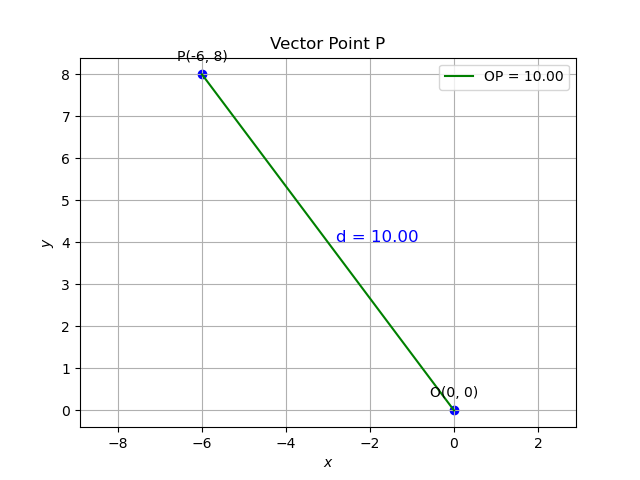
\includegraphics[width=\columnwidth]{figs/fig.png}
    \caption*{Point P\brak{-6,8}}
    \label{fig:fig}
\end{figure}

\end{document}